\documentclass[a4paper]{article}
%~~~~~~~~~~~~~~~~~~~~~~~~~~~~~Packages~~~~~~~~~~~~~~~~~~~~~~~~~~~~%
\usepackage[english]{babel}
\usepackage[utf8x]{inputenc}
\usepackage{booktabs}
\usepackage{tabu}
\usepackage{cancel}
%% Sets page size and margins
\usepackage[a4paper,top=2cm,bottom=2cm,left=2cm,right=2cm,marginparwidth=1.75cm]{geometry}
\usepackage{amsmath}
\usepackage{enumitem}
\usepackage{listings}
\usepackage{subfigure}
\usepackage{relsize}
\usepackage{graphicx}
%\usepackage{apacite}
\usepackage{pgfplots}
\usepackage[colorinlistoftodos]{todonotes}
\usepackage[colorlinks=true, allcolors=blue]{hyperref}

%~~~~~~~~~~~~~~~~~~~~~~~~~~~~~Commands~~~~~~~~~~~~~~~~~~~~~~~~~~~~%

\renewcommand{\abstractname}{Summary}

%~~~~~~~~~~~~~~~~~~~~~~~~~~~~~pgfPlots~~~~~~~~~~~~~~~~~~~~~~~~~~~~%

\pgfplotsset{compat=1.8}
\usepgfplotslibrary{statistics}
%%%%%%%%%%%%%%%%%%%%%%%%%%%%%%%%%%%%%%%%%%%%%%%%%%%%%%%%%%%%%%%%%%%%

\begin{document}

\begin{titlepage}
\begin{center}
\vspace{3cm}

\huge

\vspace{2cm}


\includegraphics[scale=0.3]{Cherubino.jpg}

\vspace{2.5cm}

{\Huge \sc Data mining project report}

\vspace{1cm}

Maddalena Amendola

\vspace{1cm}

Daniele Gadler

\vspace{1cm}

Riccardo Manetti

\vspace{1cm}

Gemma Martini

\vfill

\today

\end{center}
\end{titlepage}

%%%%%%%%%%%%~~~~~~~~~~~~~~~~~~~~~~~~~~~~~~~~~~~~~~~~~~~%%%%%%%%%%%%

\tableofcontents
\newpage

%%%%%%%%%%%%%%~~~~~~~~~~~~~~~~~~~~~~~~~~~~~~~~~~~~~~~~~~~%%%%%%%%%%
%\author{  Group 1\\ Amendola Maddalena, Daniele Gadler, Gemma Martini, Riccardo Manetti  \\Department of Computer Science, University of Pisa \\ \date{ 1nd Semester of Academic Year 2018--2019}

%\begin{abstract}
 %  This is the abstract text
%\end{abstract}


\section{Data Understanding}

This is a test

\subsection{BoxPlot by Gemma}

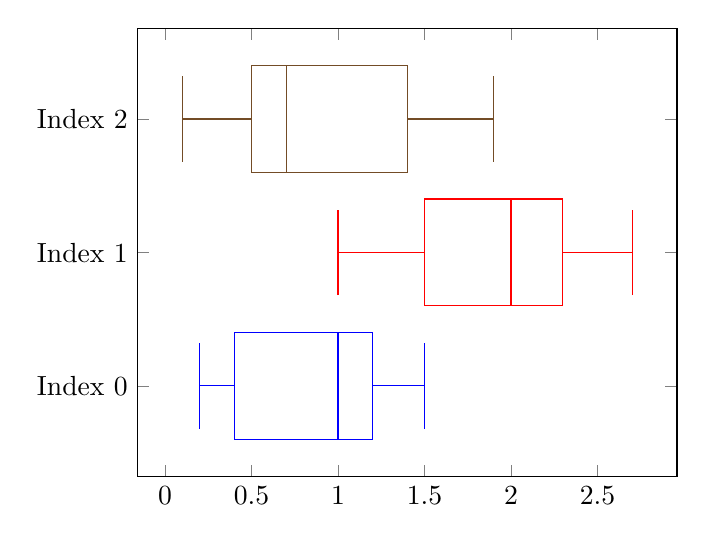
\begin{tikzpicture}
  \begin{axis}
    [
    ytick={1,2,3},
    yticklabels={Index 0, Index 1, Index 2},
    ]
    \addplot+[
    boxplot prepared={
      median=1,
      upper quartile=1.2,
      lower quartile=0.4,
      upper whisker=1.5,
      lower whisker=0.2
    },
    ] coordinates {};
    \addplot+[
    boxplot prepared={
      median=2,
      upper quartile=2.3,
      lower quartile=1.5,
      upper whisker=2.7,
      lower whisker=1
    },
    ] coordinates {};
    \addplot+[
    boxplot prepared={
      median=0.7,
      upper quartile=1.4,
      lower quartile=0.5,
      upper whisker=1.9,
      lower whisker=0.1
    },
    ] coordinates {};
  \end{axis}
\end{tikzpicture}

\bibliographystyle{plain}
\bibliography{bibtex}

\end{document}
              
